\section{Protocol Introduction}
\label{sec:theory}
	\emph{Spread  Spectrum} is a procedure to spread a transmission over a wider frequency range. The goal is robustness and support for parallel transmissions.
	Refer to \cite{ISS} for more details.
	
	Both, \emph{FHSS} and \emph{DSSS} require the sender and receiver to be time-synchronized. 
	
	\subsection{Frequency Hopping Spread Spectrum}
		In \emph{FHSS} the frequency band $f$ is split into $N$ sub-bands $f_1,..., f_N$. Each sender gets a pseudo-random chip sequence $p_n \in [f_1,...,f_N]^n$ which is known by the sender and the receiver only.
		
		\paragraph{Slow hopping} The sender will start by taking the first sub-band from its chip sequence $p_n$ and transmit on this sub-band.
		After a defined dwell time, it takes the next sub-band from $p_n$ and continue this procedure. The dwell time $T_h$ is a multiple of the symbol time $T_s$. $T_s$ is the time during which one symbol is broadcast.
		
		\paragraph{Fast hopping} In this case the symbol time $T_s$ is a multiple of the dwell time $T_h$. During the transmission of one symbol, one or multiple hops are made. So one symbol is transmitted on multiple frequencies.
		
		\paragraph{Interference} FHSS is very robust under narrow-band interference. If one sub-channel is jammed, this will only affect part of the transmission. Any other user using the same FHSS scheme will appear as narrow-band interference.
		Broad-band interference can not be easily dealt with.
		
	
	\subsection{Direct Sequence Spread Spectrum}
		Each sender has a chip sequence $p_n \in \{-1,1\}^n, \sum p_n = 1$ known the sender and receiver only. The chip-rate $R_c$ is a multiple of the signal-rate $R_s$.
		
		\paragraph{Spreading} Before sending the data sequence $d_t$, it is multiplied point-wise with the chip-pattern resulting in the transmission data $t_x = d_t p_n$.
		Image \ref{dsss} shows an example of these steps.
		This multiplication is called \emph{spreading} because the frequency of the original data $R_s$ has been increased to the frequency of the chip pattern $R_c$. This can be seen on the right side of Figure \ref{dsss}.
		
		\paragraph{Despreading} is the inverse of the spreading operation. The received signal $r_x$ is again point-wise multiplied with the chip pattern resulting in the despread data. Since $p_n p_n = [1,...,1]$, this will return the original data $d_r = t_x p_n = d_t p_n p_n = d_t$.
		
		\paragraph{Chip pattern} The length of the chip pattern $T_c$ is either the symbol length $T_s$ (short code) or a multiple of the $T_s$ (long code).
		
		When multiple users are transmitting on the same frequency range, their pattern have to be orthogonal.
		
		\paragraph{Interference} Narrow-band interference will be spread during the despreading and have little impact on the SNR. Broad-band signals uncorrelated to the chip pattern will not be affected by the despreading and thus have a higher impact on the SNR.
		See Figure \ref{dsss_interference}.
		
		\begin{figure}
			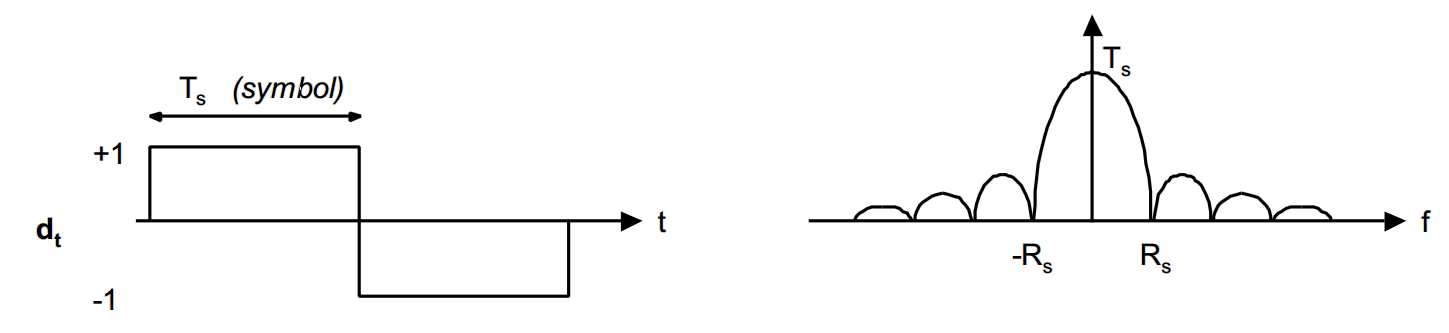
\includegraphics[width=\textwidth,keepaspectratio]{../presentation/imgs/dsss_ft_1.png}
			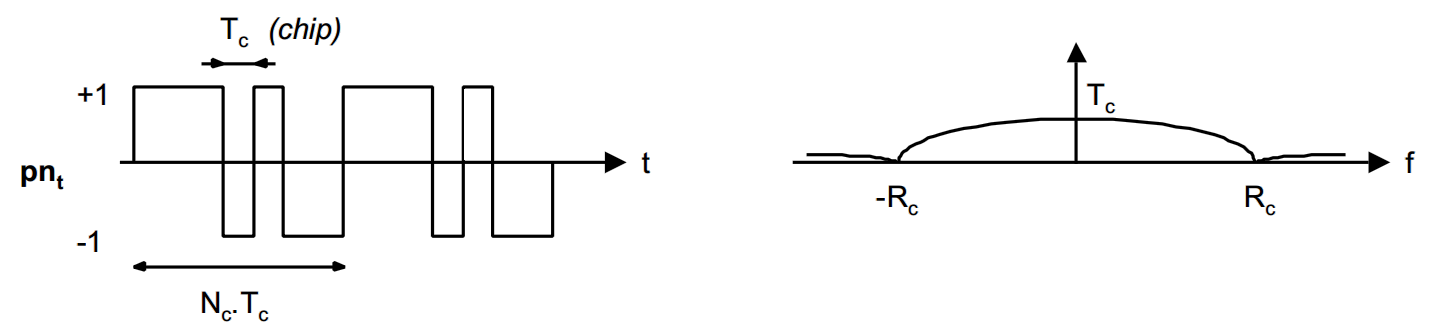
\includegraphics[width=\textwidth,keepaspectratio]{../presentation/imgs/dsss_ft_2.png}
			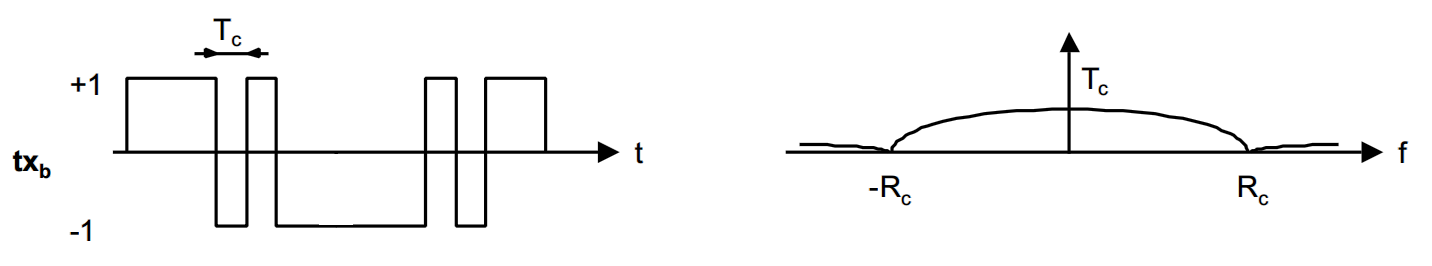
\includegraphics[width=\textwidth,keepaspectratio]{../presentation/imgs/dsss_ft_3.png}
			\caption{The spreading steps of DSSS.
					Top: Data sequence $d_t$
					Middle: Chip pattern $p_n$
					Bottom: The point-wise multiplied transmission signal $t_x = d_t p_n$
				}
			\label{dsss}
		\end{figure}
		\begin{figure}
			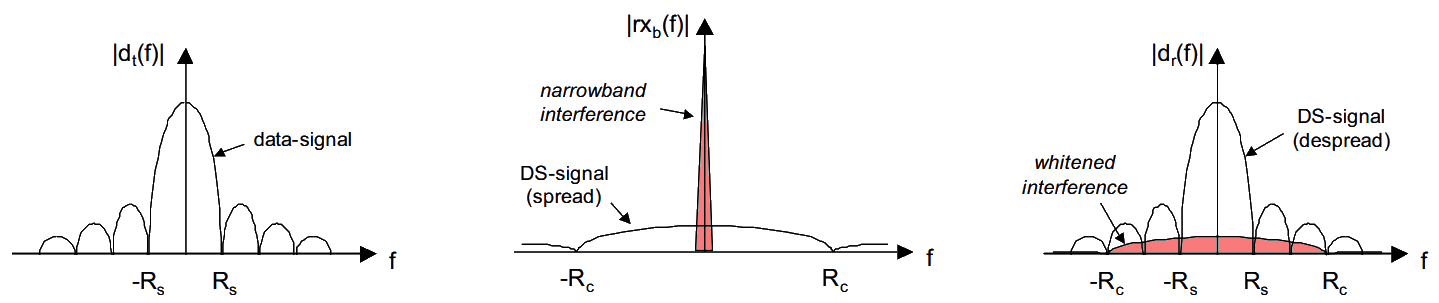
\includegraphics[width=\textwidth,keepaspectratio]{../presentation/imgs/dsss_inter_nar.png}
			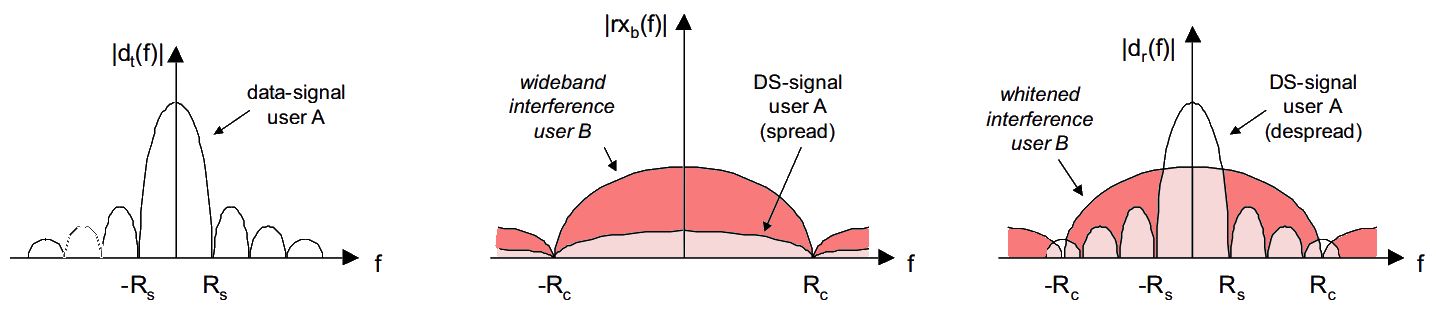
\includegraphics[width=\textwidth,keepaspectratio]{../presentation/imgs/dsss_inter_broad.png}
			\caption{ DSSS with interference.
				Top: Narrow-band interference is spread during the despreading.
				Bottom: Broad-band interference is not affected by the despreading.
				}
			\label{dsss_interference}
		\end{figure}